\documentclass[final_report.tex]{subfiles}

\begin{document}

\section{Evaluation}

This section focusses on the comparison testing which was carried out between the C and Java implementations of basic middleboxes. Evaluation of the results will then be discussed and further improvements to the Java solutions will be considered. \todo{mention machine specs} 

\subsection{Packet Generating}
Packet generating is the act of creating packets with random payloads to be sent to certain MAC addresses on the network. This can either be done via the use of specialised hardware or using software. They are used for load testing of packet processing applications to test the amount of data which applications can process per second. This can reveal whether limitations on a system is software or hardware based.

\todo[inline]{Talk about pktgen module in kernel - does dpdk version use this}

Pktgen is open source software tool, maintained by Intel, which aims to generate packets using the DPDK framework. It can generate up to 10Gbits of data per second with  varying frame sizes, and send the data in the form of packets across a compatible network interface card/controller. It has a number of benefits which include:

\begin{itemize}
	\item Real time packet configuration and port control
	\item Real time metrics on packets sent and received
	\item Handles UDP, TCP, ARP and more packet headers
	\item Can be commanded via a Lua \ref{ref this} script
\end{itemize}

\todo[inline]{how does pktgen work and why we used it, only does 32 packet bursts or less}

Pktgen's transmitting performance can be is reduced when increasing the frame size to those greater than 64 bytes. This can be negated by running the application with multiple lcores on the same port with different queues, which allow the transmitting speed to match those of the NIC. With the packet size varying, obviously the number of packets transmitted per second is depends on this. The differences are shown in Table \ref{tab:pktgen}.

\begin{table}[H]
	\centering
	\begin{tabular} { | c | c | c | }
		\hline
		\textbf{Packet Size} & \textbf{Packet/s (millions)} & \textbf{MBit/s} \\
		\hline
		64 (min) & 14.9 & 9999 \\
		\hline
		128 & 8.4 & 9999 \\
		\hline
		256 & 4.5 & 9999 \\
		\hline
		512 & 2.3 & 9999 \\
		\hline
		1024 & 1.2 & 9999 \\
		\hline
		1518 (max) & 0.8 & 9999 \\
		\hline
	\end{tabular}
	\caption{Pktgen speed at 32 packet burst, used 2 processors to get meet NIC speed}
	\label{tab:pktgen}
\end{table}

\subsection{Initial Testing}
The initial testing of applications \todo{which ones?} was carried out an a local Mac OS X machine running Ubuntu 14.04 LTS 64-bit on a VirtualBox \todo{ref this and ubuntu} virtual machine. Although this set-up didn't provide the ability to load test on very high speeds (anything above 1Gbit/s), it allowed for basic testing to check that the application was running as expected. Load testing of speeds up to roughly 700Mbit/s were also possible which have a basic testing platform without the need to move code to servers.

\subsubsection{Set-up}
Testing could be carried out using the 2 available 1Gbit NICs of the machine via a bridged network from the host to guest machine which severely reduced transmission speed. This allowed an ethernet cable to be looped back and connected between the ports, meaning anything transmitted via 1 port was guaranteed to be received by the other port.

Pktgen and the custom application were booted up simultaneously running in parallel. Careful memory allocation, port addressing and processor core assignment had to be carried out to stop shared resourced impacting the overall performance of either application. This allowed Pktgen to send packets and the application to receive and process them.

\subsubsection{Methods}

\subsubsection{Results}

\subsection{Further Testing}
In order to fully understand the capabilities of the middle boxes, testing was carried out on Imperial College's Large Scale Distributed Systems (LSDS) test-bed. Although this system consists of numerous machines, tests were carried out using just 2. The first machine was used to host the middlebox application and receive the packets. The other machine was used as the client and ran the pktgen software allowing it to generate packets at up to 10Gbps in order to take advantage of the machines network interface controllers.

The first test on the LSDS test-bed involved comparing the C and Java implementations of a packet capturing application which simply received the packets and freed them straight away without forwarding them. The C implementation is used to give the optimal readings possible from this and further tests, since very limited processing is carried out between receiving and dropping the packet. The figure below shows the performance of the application at varying packet sizes.

\missingfigure{Graph of c packet capture, 1 core, different frame sizes, will need to reference transmit speed of pktgen}

\todo{what does the results show}

The same testing was carried out with an identical packet capture algorithm which was instead implemented in Java using the DPDKJava framework described previously. These results are shown below.

\missingfigure{Graph of java packet capture, 1 core, different frame sizes, will need to reference transmit speed of pktgen}

The results above are very low to what was expected for such a simple application. \todo{expand on this}

To check where the problems lied within the code, a Java profiler (JProfiler) was used to check multiple parts of the code including memory usage, cpu usage and the number of method calls and the average time per method call. This provided invaluable analysis of where the problems were, although the profiler significantly reduced the performance of the application since it connects to the JVM and reads the data itself.

\begin{figure}
	\centering
	\begin{subfigure}{0.5\textwidth}
		\centering
		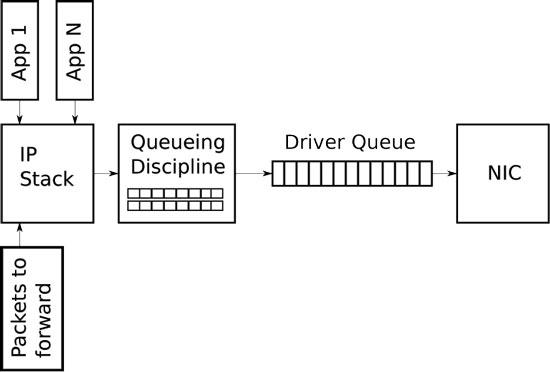
\includegraphics[width=0.5\textwidth]{img/buffer.jpg}
		\caption{fds}
		\label{sdf}
	\end{subfigure}%
	\begin{subfigure}{0.5\textwidth}
		\centering
		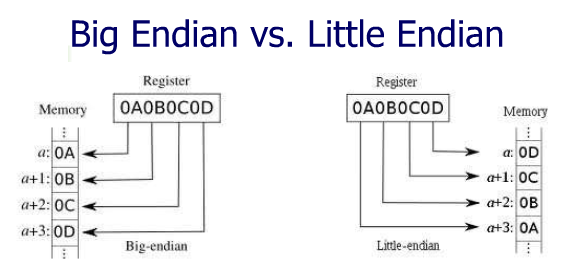
\includegraphics[width=0.5\textwidth]{img/endian.png}
		\caption{fds}
		\label{sdf}
	\end{subfigure}
	\caption{sdfd}
	\label{fdssdf}
\end{figure}

Figure ?? shows some of the output from the profiler which indicated where the main problems were in terms of memory usage and performance. From this, a number of performance upgrades were implemented:

\paragraph*{Capture Processor fields}
The first improvement were to the Packet Capture application itself. The associated processor originally stored the ReceivePoller and PacketFreeer objects within a list to allow for easy iteration if there were numerous objects. Since the Packet Capture application only used 1 of each, seperate fields could be used for the objects which removed the list accessing times and iterations.

\paragraph*{Object lifespan}
The other improvements were made to the actual DPDKJava framework. These involved utilising objects throughout the application lifespan instead of creating new ones on every loop. This dramatically reduced the number of initializing methods invoked for the objects and reduced the memory usage in the heap, which reduced the number of times the Java garbage collector was invoked. The class which caused the most problem with this was the ArrayList, which were created on every loop to pass packets through the Java system. Since the framework uses threads without the need to synchronise objects, an ArrayList could be created on initialisation and simply cleared before been used again.

\paragraph*{Off heap allocation}
Finally, instead of allocating new off heap memory to receive the packet pointers through on every loop, a memory bank was allocated on initialisation and the same memory was simply overwritten on every loop iteration. These improvements resulted in the graph below.

Again, the same tests were carried out to check the performance increase of the framework implementation.

\missingfigure{Graph for improvements}

\todo{explain results compared to previous ones and c version}

\missingfigure{more profiling?}

\paragraph*{Packet creation}
Of course, for every packet entering the application a packet object is created for easy referencing further down the application pipe-line. However, not using packet objects would significantly reduce the usability and scalability of applications. It was decided not to alter this. However, for each packet initialization a new UnsafeAccess object was been created for use with accessing packet header information. However, since each thread controls its own packets and therefore can only process 1 packet at a time, 1 UnsafeAccess object could be shared between all packets which significantly reduced the number of objects on the heap.

\paragraph*{Send and Free lists} Further problems were identified with the lists of packets awaiting to be sent and freed. This list was been iterated over with the Packet's mbuf pointer then been stored in an off heap memory bank waiting to be freed. This was pointless since the packets mbuf pointer could directly be put into the off heap memory, therefore eliminating the need for the list while also allowing the packet objects to be dereference quicker.

\todo{image of this}

\missingfigure{Graph for improvements}

The results show that the performance was further improved and pretty close to that of the C implementation. After further profiling, there was only 1 obvious improvement which could be made, This would be to replace the list storing packets received from the poller. However, replacing this with a custom implementation using off heap memory would firstly reduce the usability of the code and would also mean that the code was drifting away from the Java language. It was decided not to implement this fix and instead to continue with testing of other applications, assuming that the would be negated by applications. This initial series of testing also proved that a dramatic increase in performance can be achieved simply by programming the applications efficiently, by trying to reduce the number of objects created.

%http://www.oracle.com/technetwork/java/hotspotfaq-138619.html#perf%5Fscaling
%http://stackoverflow.com/questions/11054548/what-does-the-usecompressedoops-jvm-flag-do-and-when-should-i-use-it
%http://www.oracle.com/technetwork/systems/index-156457.html
%http://java-performance.info/various-methods-of-binary-serialization-in-java/
%http://java-performance.info/memory-allocation-in-java/
%https://wikis.oracle.com/display/HotSpotInternals/PerformanceTechniques
%http://www.ibm.com/developerworks/library/j-nativememory-linux/
%http://codedependents.com/2014/01/27/11-best-practices-for-low-latency-systems/
%http://infotechgems.blogspot.co.uk/2011/11/java-collections-performance-time.html
%http://www.javaworld.com/article/2077647/build-ci-sdlc/make-java-fast--optimize-.html
%http://vanillajava.blogspot.co.uk/2011/05/how-to-get-c-like-performance-in-java.html
%ftp://ftp.glenmccl.com/pub/free/jperf.pdf
%http://www.ibm.com/developerworks/library/j-zerocopy/
%http://www.oracle.com/technetwork/java/jvmls2014tene-2265204.pdf
%http://mechanical-sympathy.blogspot.co.uk/2012/07/native-cc-like-performance-for-java.html
%http://java-is-the-new-c.blogspot.co.uk/2014_12_01_archive.
%http://psy-lob-saw.blogspot.co.uk/2012/12/encode-utf-8-string-to-bytebuffer-faster.html
%http://stackoverflow.com/questions/145110/c-performance-vs-java-c
%http://stackoverflow.com/questions/2163411/is-java-really-slow
%http://mechanical-sympathy.blogspot.de/2012/07/native-cc-like-performance-for-java.html
%https://blogs.oracle.com/moonocean/entry/a_simple_example_of_jni
%http://zeroturnaround.com/rebellabs/dangerous-code-how-to-be-unsafe-with-java-classes-objects-in-memory/
%http://java.dzone.com/articles/understanding-sunmiscunsafe
%http://www.techrepublic.com/article/discover-how-the-java-native-interface-works/
%http://mishadoff.com/blog/java-magic-part-4-sun-dot-misc-dot-unsafe/
%https://people.kth.se/~danieltt/pktgen/docs/DanielTurull-thesis.pdf

\subsubsection{Set-up}

\subsubsection{Methods}

\subsubsection{Results}

\subsection{Software Design}
Mention somewhere about the limitations of pktgen

\subsubsection{Portability}

\subsection{Possible Improvement}

\end{document}